%!tikz editor 1.0
\documentclass{article}
\usepackage{tikz}
\usepackage[graphics, active, tightpage]{preview}
\usetikzlibrary{intersections}
\usetikzlibrary{shapes}
\usetikzlibrary{chains}
\graphicspath{ {cisco-icons-bw-eps/} }
\PreviewEnvironment{tikzpicture}

%!tikz preamble begin

%!tikz preamble end


\begin{document}
%!tikz source begin
\begin{tikzpicture}[
    start chain=going right,
    diagram item/.style={
        on chain,
        join
    }
]
\node [
    diagram item,
    label=center:Internet
] {
\includegraphics{cloud}};
\node [
    diagram item,
    label=right:Cable Modem
] {
\includegraphics{cable_modem}};

\node [
    continue chain=going below,
    diagram item,
    label=right:Router
] {
\includegraphics{router}};
\node [
    diagram item,
    label=right:Workgroup Switch
] {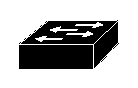
\includegraphics{workgroup_switch}};

\node [
    start branch=1 going below right,
    diagram item,
    label=below:PC
] {
\includegraphics{pc}};

\node [
    start branch=2 going below left,
    diagram item,
    label=below:Supercomputer
] {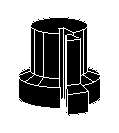
\includegraphics{supercomputer}};

\node [
    diagram item,
    label=below:Office
] {\includegraphics{end_office}};
\end{tikzpicture}
%!tikz source end

\end{document}